%%%%%%%%%%%%%%%%%%%%%%%%%%%%%%%%%%%%%%%%%%%%%%%%%%%%%%%%%%%%%%%%%%%%%%%%%
%                           Marco Conceptual                               %
%%%%%%%%%%%%%%%%%%%%%%%%%%%%%%%%%%%%%%%%%%%%%%%%%%%%%%%%%%%%%%%%%%%%%%%%%

\chapter{Desarrollo del Sitema}\label{chapter5}

En este capitulo se cubre el desarrollo del sistema descrito en capítulos anteriores tomando como referencia los casos de uso, abarcando cada uno de los módulos que lo componen.

\section{Módulo del Microcontrolador}

\subsection{Objetivo}
El caso de uso \ref{SUB-M-CU1.3} nos indica que el microcontrolador debe consultar el dispositivo de adquisicion MCP39F521 para conseguir el valor de potencia activa por medio del protocolo IIC, para lograr esta tarea, nos apoyamos en las hojas de datos de los fabricantes, debemos programar el microcontrolador DSPIC30F4013, para ello ocupamos el entorno de desarrollo del fabricante (mplab de Microchip) para crear un proyecto en lenguaje C e interfaz con ensamblador, el entorno de desarrollo de microchip facilita la programación de sus microcontroladores gracias a que tiene bibliotecas y compiladores listos para usarse.

\subsection{Configurando conexión con el dispositivo de adquisición}
Lo primero que debemos conocer es cual es el registro de control de IIC en el microcontrolador, esto podemos encontrarlo en la hoja técnica del microcontrolador, el registro de control, entre otras funciones, habilita la comunicación IIC, configura la velocidad del reloj IIC, recordando que es un protocolo de transmisión de información síncrona por el uso de una linea de reloj, que en la hoja técnica del dispositivo de adquisición nos indica que es de 400KHz.

\paragraph{}
Una ves configurados esos dos parámetros, físicamente solamente necesitamos conectar los pines de SDA (linea de datos), SCL (linea de reloj), VCC y GND de ambos, este dispositivo de adquisición ya contiene en sus registros los valores de potencia, voltaje y corriente entre otros, que son convertidos y acondicionados automáticamente con el ADC y Filtro Digital que tiene integrado como se muestra en la figura \ref{fig:Diagrama funcional} .

\begin{figure}[H]
	\centering
	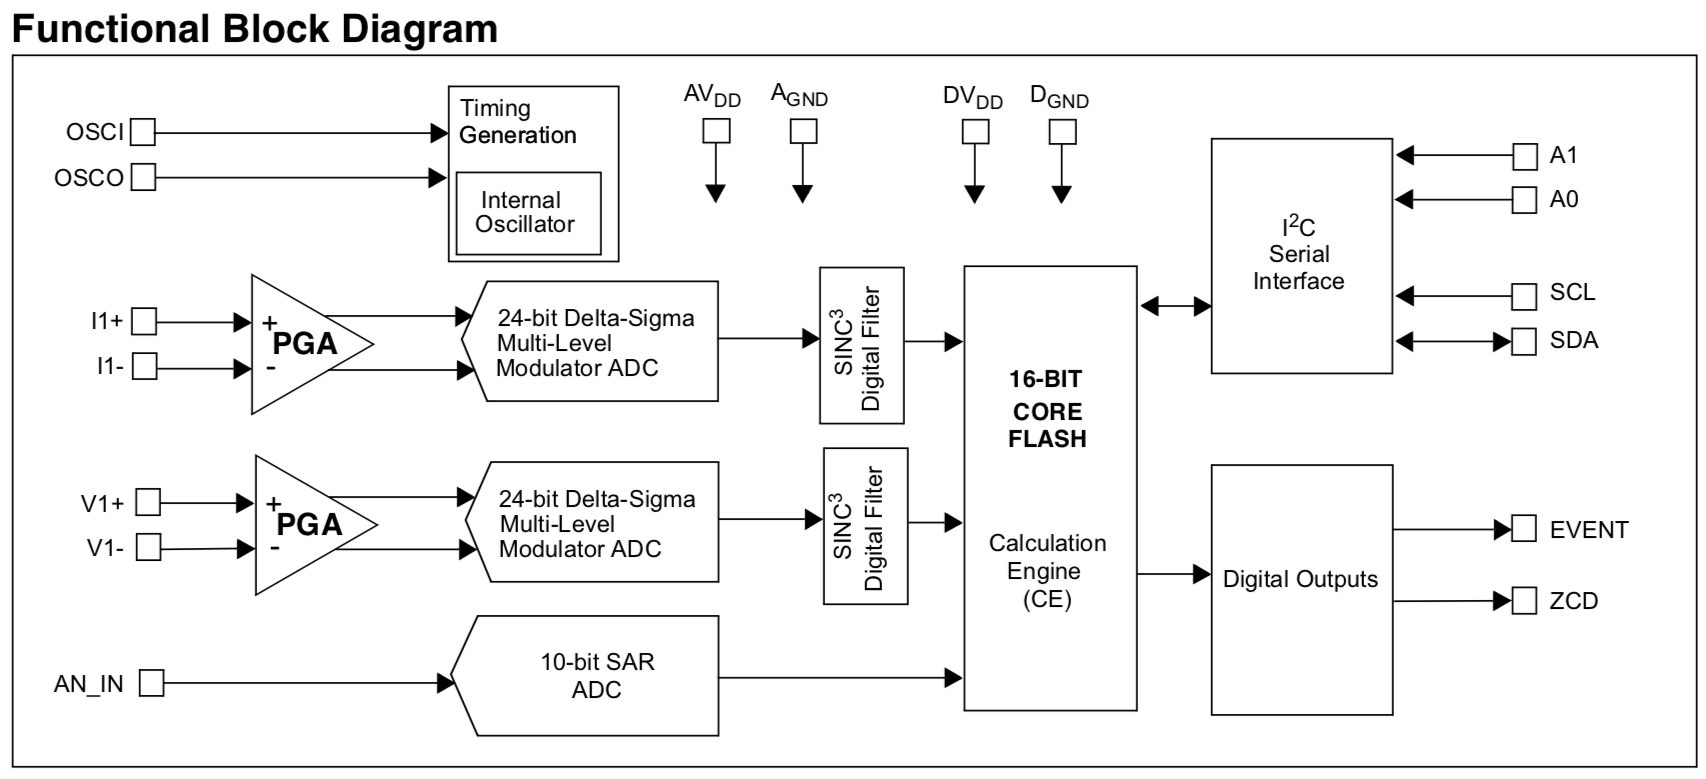
\includegraphics[scale=.4]{Capitulo5/images/MCP_diagrama_funcional.png}
	\caption{Diagrama funcional del dispositivo de adquisición}
	\label{fig:Diagrama funcional}
\end{figure}

\begin{figure}[H]
	\centering
	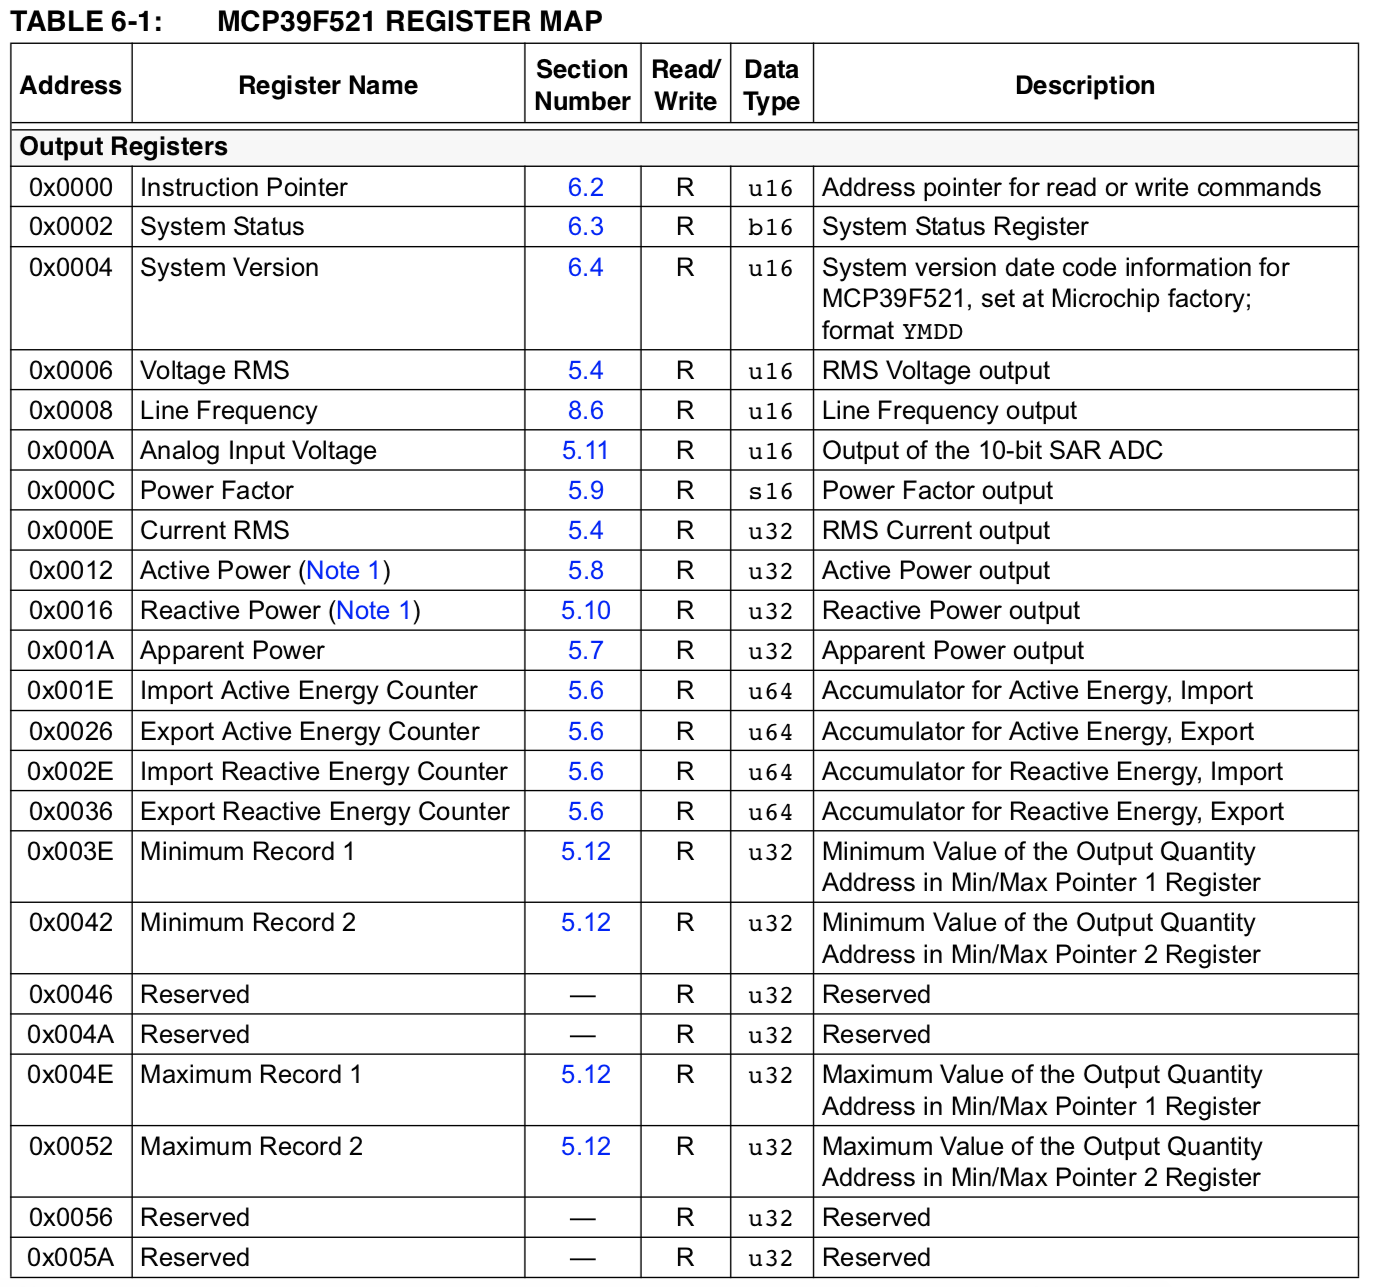
\includegraphics[scale=.5]{Capitulo5/images/register_map.png}
	\caption{Mapa de registros del MCP39F521}
	\label{fig:Mapa de registros del MCP39F521}
\end{figure}

\subsection{Comunicación con el dispositivo de adquisición vía software}

La comunicación IIC con el dispositivo de adquisicion se realiza, principalmente con los siguientes comandos definidos por el protocolo:

\begin{enumerate}
    \item Inicio de comunicación (START)
    \item Fin de comunicación (STOP)
    \item Acuse de recibo (ACK)
    \item No acuse de recibo (NACK)
    \item Envió de información
    \item Recibo de información
\end{enumerate}

Estas funciones ya están implementadas en lenguaje ensamblador, en una biblioteca denominada I2C.s y nosotros las ocupamos en el programa principal en lenguaje C por medio de su declaración global, en el código siguiente se muestran las rutinas para el comando de inicio de comunicación y envió de datos.

\begin{lstlisting}[language={[x86masm]Assembler}]

;****DECLARACION DE METODOS GLOBALMENTE PARA SU USO EN C*****
.GLOBAL	_START_I2C
.GLOBAL	_ENVIA_DATO_I2C

;************************************************************
ESTA RUTINA GENERA LA CONDICION DE START AL BUS I2C
ENVIANDO CON EL REGISTRO DE CONTROL AL ESCLAVO LA SEÑAL
Y ESPERANDO SU RESPUESTA
;************************************************************
_START_I2C:
	BCLR		IFS0,			#MI2CIF
	BSET		I2CCON,			#SEN
ESPERA_START:
	BTSS		IFS0,			#MI2CIF
	GOTO		ESPERA_START

	RETURN
	
;************************************************************
ESTA RUTINA GENERA LA CONDICION DE ENVIO DE DATO AL BUS I2C
EN ESTE CASO, COPIAMOS LO QUE ESTA EN EL REGISTRO W0 AL 
REGISTRO DE TRANSMISION DE I2C ESPERANDO LA RESPUESTA DEL
ESCLAVO
;************************************************************
_ENVIA_DATO_I2C:
	BCLR		IFS0,			#MI2CIF
	MOV.B		WREG,			I2CTRN
ESPERA_ENVIA_DATO_I2C:
	BTSS		IFS0,			#MI2CIF
	GOTO		ESPERA_ENVIA_DATO_I2C
	
	RETURN
	
\end{lstlisting}

\subsection{Escritura de comandos para el dispositivo de adquisición}

En la figura \ref{fig:Comando de escritura} se muestra la estructura de un byte de control para la escritura de un comando, con un bit de inicio, un byte de control que indica hacia qué dispositivo nos dirigiremos, A1 y A0 son los bits de direccionamiento, podemos dirigirnos hacia 4 diferentes esclavos, en este caso al tener solo uno, la dirección será “00”, seguido del bit que indica si será una operación de lectura o escritura, al ser escritura toma el valor de cero, formando como byte de control “11101000”.

\begin{figure}[H]
	\centering
	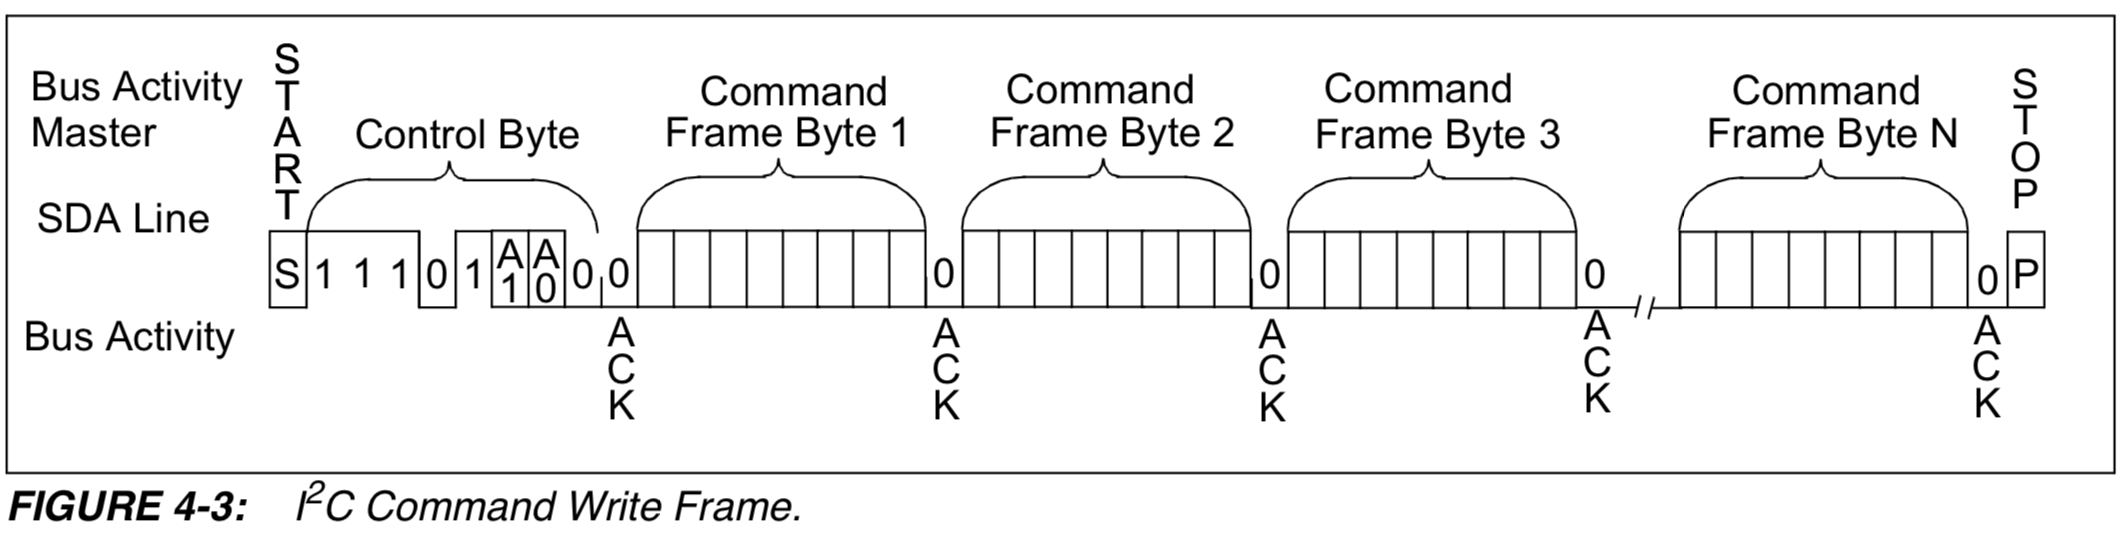
\includegraphics[scale=.4]{Capitulo5/images/write_command.png}
	\caption{Comando de escritura de comando para el dispositivo de adquisición MCP39F521}
	\label{fig:Comando de escritura}
\end{figure}

El byte de control, indica al dispositivo de adquisición que vamos a iniciar una lectura, este es seguido por un marco o marcos de comandos a ejecutar como sse muestra en la figura \ref{fig:Marco de escritura de lectura} , están compuestos por una cabecera, cuantos bytes se recibirán, el o los comandos a ejecutar y un checksum para verificar que la información llego completa y correcta, éste se calcula sumando los datos mencionados y dividiéndolos entre 256, el residuo de esta división es el checksum.

\begin{figure}[H]
	\centering
	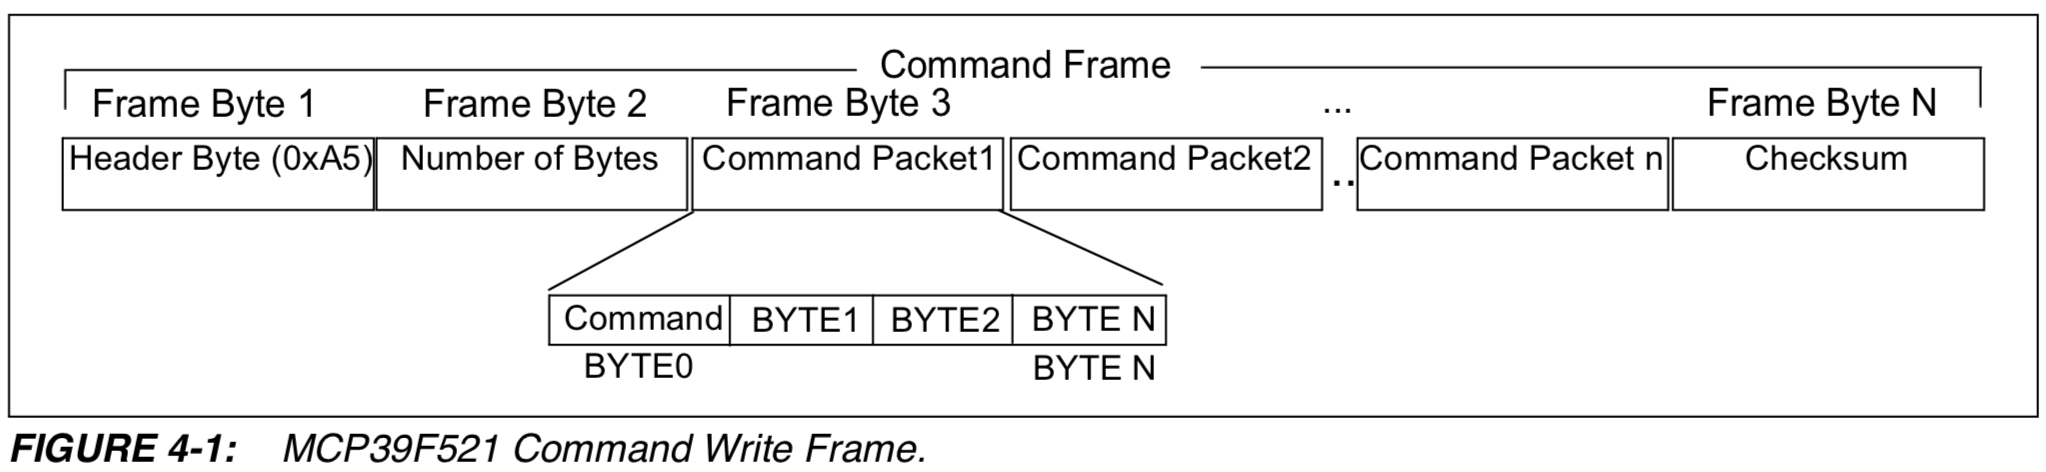
\includegraphics[scale=.4]{Capitulo5/images/marco_write_command.png}
	\caption{Marco lectura}
	\label{fig:Marco de escritura de lectura }
\end{figure}

Traducido a código en lenguaje c, la rutina que escribe un comando de lectura de registro se ve de la siguiente forma:

\begin{lstlisting}[language=C]

unsigned char enviaComando ( 
  unsigned char direccion, unsigned char registro, 
  unsigned char bytes, unsigned char checksum )
{
    START_I2C();
 
    //Control byte, write command
    
    ENVIA_DATO_I2C(direccion); //11101000   
    
    if( I2CSTATbits.ACKSTAT == 1 ){ //NACK del sensor
        return NANCK;
    }

    // Inicio del I2C Command Write Frame.
    
    ENVIA_DATO_I2C(0xA5); //header byte
        
    ENVIA_DATO_I2C(0x08); //no. bytes in frame
    
    ENVIA_DATO_I2C(0x41); //command set address pointer
   
    ENVIA_DATO_I2C(0x00); //addr high
     
    ENVIA_DATO_I2C(registro); //addr low 

    ENVIA_DATO_I2C(0x4E); //command read register
    
    ENVIA_DATO_I2C(bytes); //number of bytes to read 
    
    ENVIA_DATO_I2C(checksum); //checksum   
   
    if( I2CSTATbits.ACKSTAT == 1 ){ //NACK del sensor
        return NANCK;
    }
          
    STOP_I2C();
    return EXITO;
}

\end{lstlisting}

\subsection{Lectura de respuesta del dispositivo de adquisición}

Ahora que logramos comunicarnos con el sensor para requerir la lectura de su o sus registros, necesitamos conocer la respuesta resultante, para ello tenemos que seguir el formato del byte de control de lectura de respuesta del dispositivo esclavo que el fabricante indica en la figura \ref{fig:Comando de lectura de respuesta} , tiene un bit de inicio, un byte de control, que nos indica a qué dispositivo esclavo nos dirigimos, en este caso una vez más al “00”, seguido del bit que indica si será una operación de lectura o escritura, al ser lectura toma el valor de uno, formando como byte de control “11101001” seguido de los marcos de respuesta.

\begin{figure}[H]
	\centering
	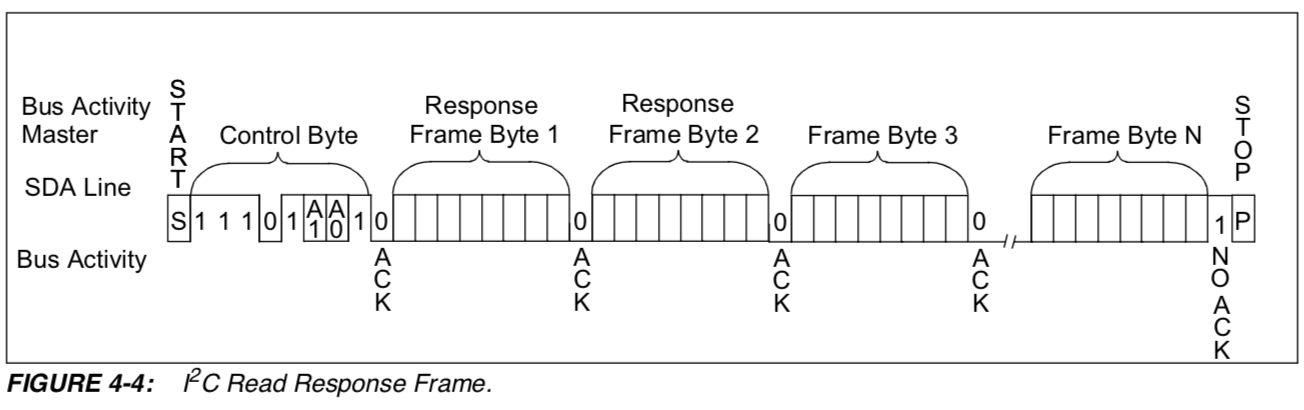
\includegraphics[scale=.7]{Capitulo5/images/read_command.png}
	\caption{Comando de lectura para el dispositivo de adquisición MCP39F521}
	\label{fig:Comando de lectura de respuesta}
\end{figure}

Después del envió del byte de control, recibimos los marcos de respuesta que se muestran en la figura \ref{fig:Marco de respuesta del Dispositivo de Adquisición MCP39F521} , que nos indican un acuse especial con valor de 6 hexadecimal, seguido de el numero de bytes que lo conforman, los bytes de información y finalmente un checksum.

\begin{figure}[H]
	\centering
	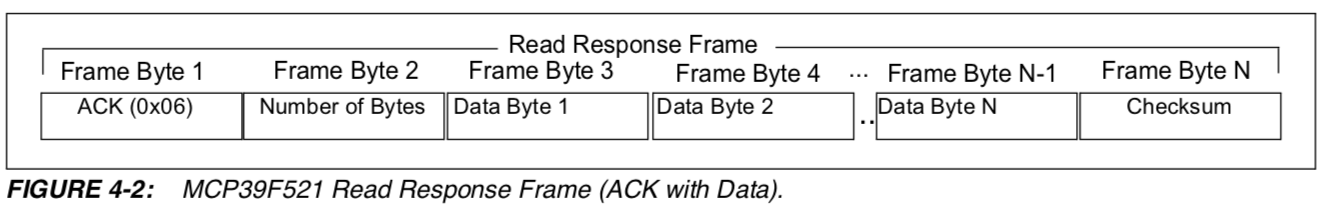
\includegraphics[scale=.7]{Capitulo5/images/responde_frame.png}
	\caption{Marco de respuesta para el dispositivo de adquisición MCP39F521}
	\label{fig:Marco de respuesta del Dispositivo de Adquisición MCP39F521}
\end{figure}

Traducido a código en lenguaje c, la rutina que escribe un comando de lectura de respuesta se ve de la siguiente forma:

\begin{lstlisting}[language=C]

unsigned char leeRespuesta(unsigned char direccion)
{   
    
    START_I2C();
    
    //control byte, read response
    
    ENVIA_DATO_I2C(direccion+0x01); //11101001   
    
    if( I2CSTATbits.ACKSTAT == 1 ){ //NACK del sensor
        return NANCK;
    }

    //ack (0x06)
    RECIBE_DATO_I2C();
    ACK_MST_I2C();
    
    //number of bytes 
    int no_bytes = RECIBE_DATO_I2C();
    ACK_MST_I2C();
    
    int i;
    
    //data bytes
    for(i = 0 ; i < no_bytes-3 ; i++){
        U2TXREG = RECIBE_DATO_I2C();
        ACK_MST_I2C();
    }
    
    //checksum
    RECIBE_DATO_I2C();
    NACK_MST_I2C();
    
    STOP_I2C();  
    return EXITO;
}

\end{lstlisting}

\subsection{Envío de muestras al servidor vía Wi-Fi}

Con estas éstas dos rutinas, conseguimos en bytes, la información del voltaje, corriente, factor de potencia, frecuencia, potencia aparente, activa y reactiva de un panel solar, estos bytes los enviamos por medio del módulo Wi-Fi por medio de la interfaz de comunicación UART, la conexión física de este módulo Wi-Fi es senculla, usa un estandarde pines para su montura llamado mikrobus \ref{fig:Mikrobus}, que principalmente tiene un transmisor (TX), receptor (RX), ChipSelect (CS) así como GND y VCC. 


\begin{figure}[H]
	\centering
	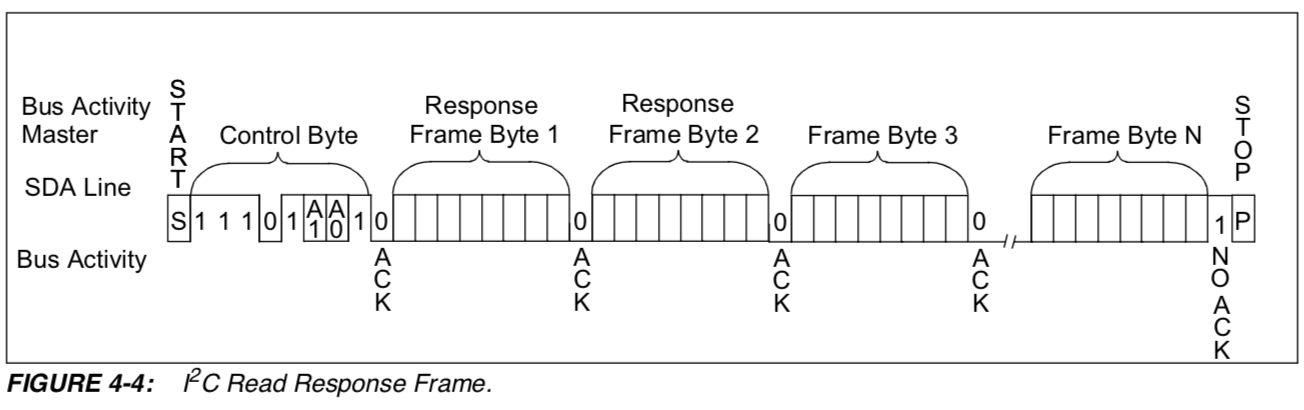
\includegraphics[scale=.7]{Capitulo5/images/read_command.png}
	\caption{Estándar de Pines Mikrobus}
	\label{fig:Mikrobus}
\end{figure}

Para poder usar el modulo WiFi a nivel programación, debemos primero, configurar sus los registros de configuración del modulo UART, el MCP30F4013 tiene 2 interfaces UART, pero la segunda es la que tiene el acomodo para el estándar mikrobus, debemos activar la interfaz UART, configurar la velocidad de transición de información, esto se calcula dividiendo la frecuencia de trabajo de nuestro microcontrolador (1.8*10\^6) entre el Baudaje del modulo Wi-FI, que es de 115200 Baudios.

Después, debemos configurar las interrupciones, de manera que cuando se coloque un dato en el registro que envia datos del modulo Wi-Fi, este automáticamente lo envíe.


\begin{lstlisting}[language=C]

void iniprograma(){
    
    CONTRX = 0;
    
    iniPerifericos();
    
    //UART2 BAUDIOS:115200 mikrobus2 (WIFI)
    U2MODE = 0X0020; //uart disable ,no usa los alternos, autobaudaje
    U2STA  = 0X8000;
    U2BRG  = 0; // (1.8432*10^6)/(16*115200) = 0

    //Interrupciones de uart2 (Modulo wifi))
    IFS1bits.U2RXIF= 0;
    //U2RX interrupts ENABLE
    IEC1bits.U2RXIE= 1;
    
    //Habilitamos el uart2 (Modulo wifi)
    U2MODEbits.UARTEN = 1;
    U2STAbits.UTXEN = 1;
    
    //habilitando el registro de control sensor
    I2CCONbits.I2CEN = 1;
    
    //Inicializamos el modulo wifi
    iniWIFI();
    configWIFI();
}

\end{lstlisting}

Lo que prosigue una vez configurada la comunicación UART con el módulo Wi-Fi, es configurar la red del mismo, esto se realiza con comandos AT, dónde configuramos la red a la que nos conectaremos, el protocolo de envió de paquetes, en este caso UDP, a que IP y Puerto nos dirigimos, donde indico la dirección del servidor y cuantos bytes de información se enviaran.

\begin{lstlisting}[language=C]
//Configuracion del modulo WIFI
void configWIFI(void){  
    
    comandoAT("ATE0\r\n"); //echo off
    sendOK();
    comandoAT("AT+RST\r\n");
    sendOK();
    comandoAT("AT+CWMODE=1\r\n"); //wifi-mode: softAP + station mode
    sendOK();
    comandoAT("AT+CIPMUX=0\r\n"); //disable multiple connections
    sendOK();
    comandoAT("AT+CWJAP=\"CELECSIS\",\"PIC18f2550\"\r\n");
    sendOK();
    comandoAT("AT+CIFSR\r\n"); //get local ip address 
}

//Envio de paquetes
void enviaWIFI(void){
    
    comandoAT("AT+CIPSTART=\"UDP\",\"104.198.212.166\",4000\r\n");
    sendOK();
    comandoAT("AT+CIPSEND=21\r\n");
    sendOK();
    
    //---Colocar aquí los nodos existentes---//
    
    //---Enviando numero de serie de microcontolador (AA)
    numero de sensor (0) y su informacion ---//
    U2TXREG = 'A';
    U2TXREG = 'A';

    U2TXREG = 0x00;

    leeTransmiteSensor(0xE8);
    sendOK();
    //----------------------------------------//   
    
    
    comandoAT("AT+CIPCLOSE\r\n");
    sendOK();
    
}
\end{lstlisting}

En la función principal, se envían muestras al servidor, no exactamente cada segundo, hicimos pruebas y cubre 50 muestras al minuto y hacemos un reinicio cada 30 minutos por si hay algún tipo de falla con la conexión de red.

\begin{lstlisting}[language=C]
//programa principal
int main (void)
{     
    iniprograma();

    //reinicio del programa cada media hora
    int counter = 0;
    
    //enviamos muestras cada segundo y reiniciamos el sistema cada media hora
    for(;EVER;)
    {           
        enviaWIFI();
        
        counter = counter+1;
        
        if(counter == 900){
            iniprograma();
            counter = 0;
        }
        
        __delay_ms(500);
    }
    
    return 0;
}
\end{lstlisting}

\subsection{Resultado final}

Físicamente, la figura \ref{fig:conexion hardware} muestra como se hace la conexión entre microcontrolador con dispositivo de adquisición, el montaje del modulo Wi-Fi, la conexión del panel solar a la carga y su inyección a la linea eléctrica.
    
\begin{figure}[H]
	\centering
	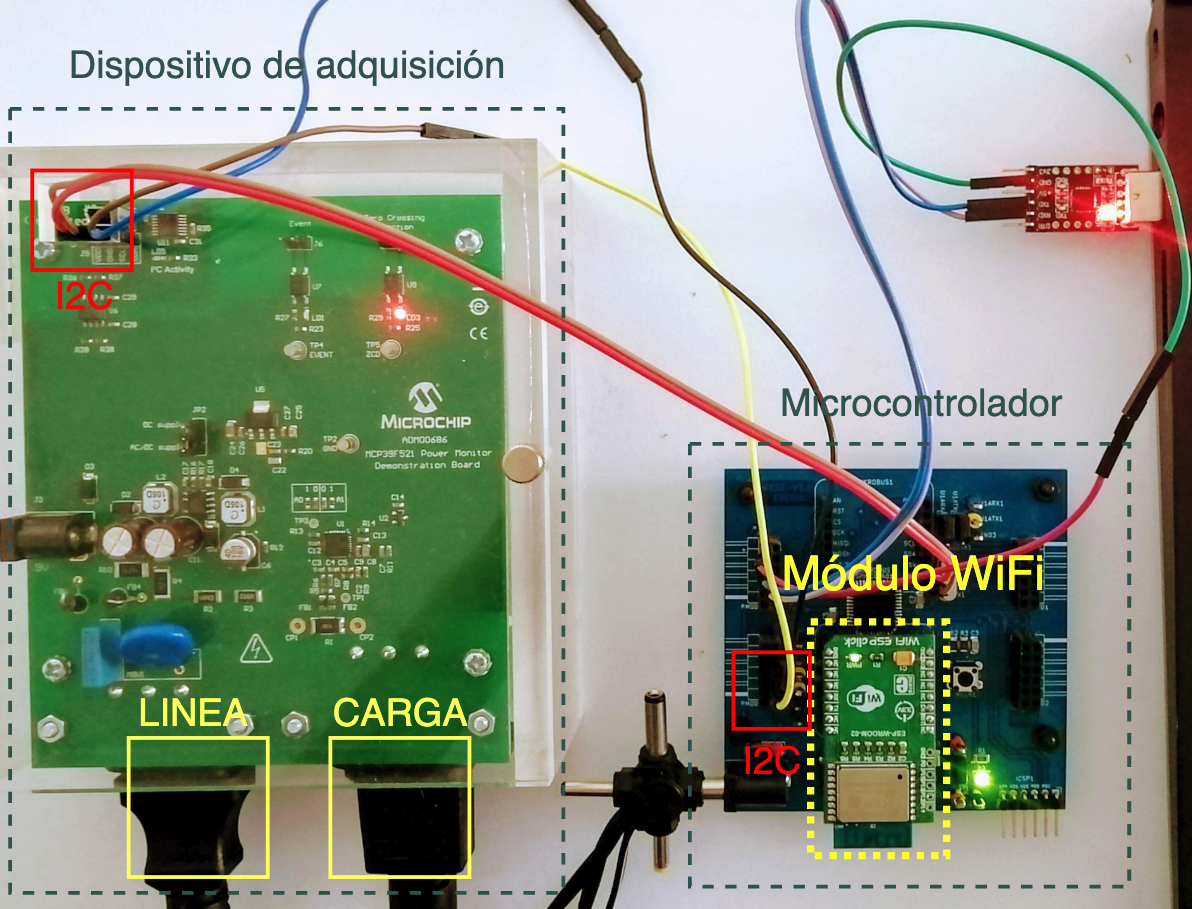
\includegraphics[scale=.3]{Capitulo5/images/conexion_fisica.png}
	\caption{Conexión de hardware del sistema}
	\label{fig:conexion hardware}
\end{figure} 

Para probar el funcionamiento de la comunicación con el dispositivo de adquisición via IIC, se conecto un cable USB con comunicación UART al microcontrolador, que copia los mismos datos que se envían al modulo Wi-Fi, a una computadora, solamente agregamos los pines del UART1 en la configuración del programa y copiamos en su registro de transmisión los datos conseguidos, nos basamos en el ejemplo de la hoja técnica para comparar el resultado conseguido.

\begin{figure}[H]
	\centering
	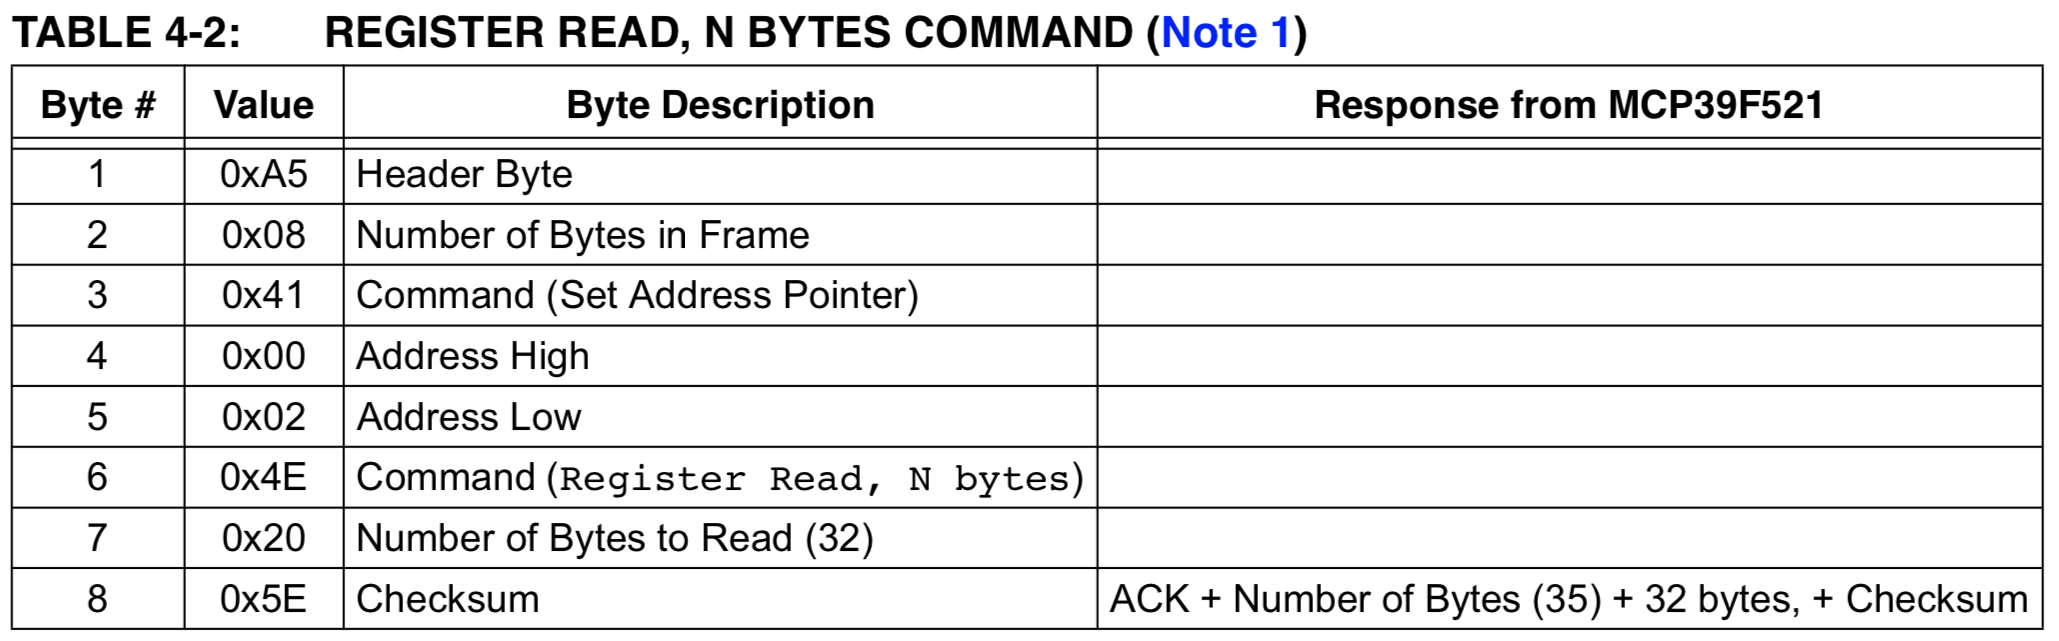
\includegraphics[scale=.3]{Capitulo5/images/respuesta_sensor.png}
	\caption{Respuesta del sensor a un comando de lectura determinado}
	\label{fig:respuesta sensor}
\end{figure} 

En la consola de la computadora, vemos la siguiente información impresa en pantalla,  podemos interpretarla de la siguiente forma:

\begin{itemize}
    \item Los dos primeros valores 255 nos marcan el fin de la transmisión
    \item ACK de la respuesta del esclavo (6 en ascii).
    \item Número de bytes (35)
    \item Los siguientes 32 datos son los datos enviados por el dispositivo esclavo del estado del sistema segun el mapa de registros \ref{fig:Mapa de registros del MCP39F521} .
    \item El 170 es el checksum del envío de la trama, podemos comprobarlo sumando desde el valor del acuse (6) hasta el penúltimo dato, dando un total de 1706 decimal, si dividimos esto entre 256, el valor del checksum será igual al residuo de la división, que es igual a 170.
\end{itemize}

\begin{figure}[H]
	\centering
	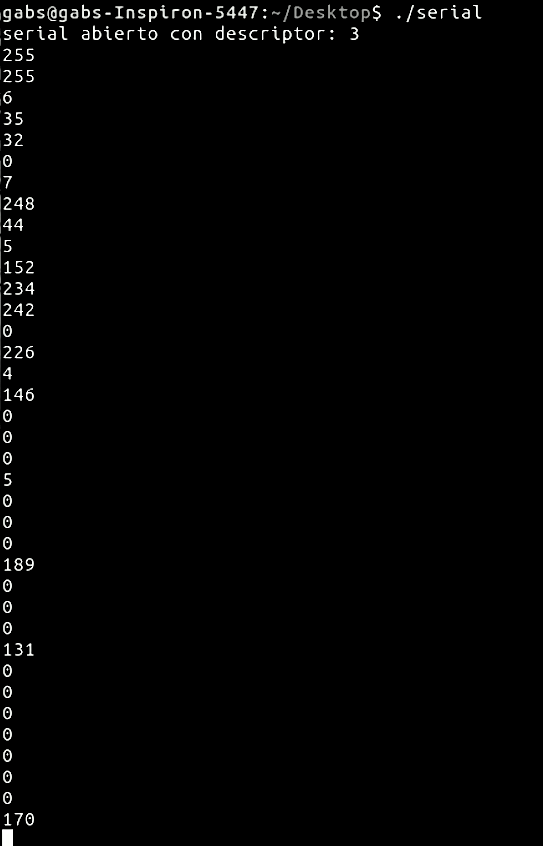
\includegraphics[scale=.3]{Capitulo5/images/consola.png}
	\caption{R}
	\label{fig:consola}
\end{figure} 

La ultima funcionalidad por probar es el envió de muestras al servidor, lo único que tenemos que hacer, es crear un servidor UDP en la IP y Puerto indicados en el programa del microcontrolador para la captura de los paquetes:


\begin{lstlisting}[language=Python]
import socket
import sys
import datetime, time
import os
import struct

#---------------Variables de configuracion-----------------
server_ip = '10.128.0.2'
port = 4000
#----------------------------------------------------------

# Creando socket UDP
sock = socket.socket(socket.SOCK_DGRAM, socket.SOCK_DGRAM)

# Relacionar direccion IP con puerto
server_address = (server_ip, port)
sock.bind(server_address)

print ('Starting up server on %s port %s' % server_address)

# Esperando por conexion
while True:

    print('Waiting for a connection...')
    
    pack, client_connection = sock.recvfrom(21)

    #Recibiendo paquete de 21 bytes
    pack = struct.unpack('21B',pack)

    packet = pack

    #Imprimir paquete recibido
    print(packet)

\end{lstlisting}

Y el resultado de este programa, es la captura de paquetes que tienen una longitud de 21 Bytes:

Byte 1 y 2: El numero de serie del microcontrolador en código ASCII

Byte 3: El numero de esclavo en valor decimal

Byte 4 y 5 : El valor del voltaje actual, esta dividido en dos bytes, consiguiendo el byte menos significativo, de esta forma conseguimos un valor flotante.



